\section{Overview}

The aim of Shimmer++ development is to build an efficient open-source tool in C++ for the numerical modelling of natural gas transport through a long-distance network. Shimmer++ is capable of steady and unsteady state simulations with mixture of gases, to take into account - for instance -  hydrogen blending. Other open-source tools exist, to mention some: GasNetSim, pandapipes and MORGEN. The first was presented recently in \url{https://ieeexplore.ieee.org/document/9769148}, where authors argued GasNetSim is the first open-source tool that allows complex mixture composition of gases. This salient advantage can be only exploited for steady regime. The second library has less model flexibility and, as in in the former, is written Python. The latter stands for Model Reduction for Gas and Energy Networks, which is an academic tool developed in Matlab based on the isothermal Euler equations. \cred{[CONTRIBUTION REQUIRED FROM DENERG]}  

Shimmer++ is a purely computational tool mainly intended to interact with other software, for example GIS programs. Therefore, Shimmer++ does not provide any user interface and the interaction is purely file-based.

%\subsection{Architecture of shimmer++} 
The Shimmer++ tool is based on the architecture shown in Fig. \ref{intro:architecture}. The main functional domains are the on-disk gas network representation, the in-memory representation, and the numerical methods operating on the networks. From the users' point of view this three-layer architecture translates to the following:
\begin{itemize}
    \item the on-disk representation is realized by the the Network Data Files (NDFs), which are SQLite databases where the gas networks are stored and are the main interaction mechanism between Shimmer++ and the user (where the user is potentially another software)
    \item the in-memory representation and the numerical methods layer are the actual shimmer++ tool, which reads and writes NDFs
\end{itemize}

\begin{figure}[H]
    \centering
    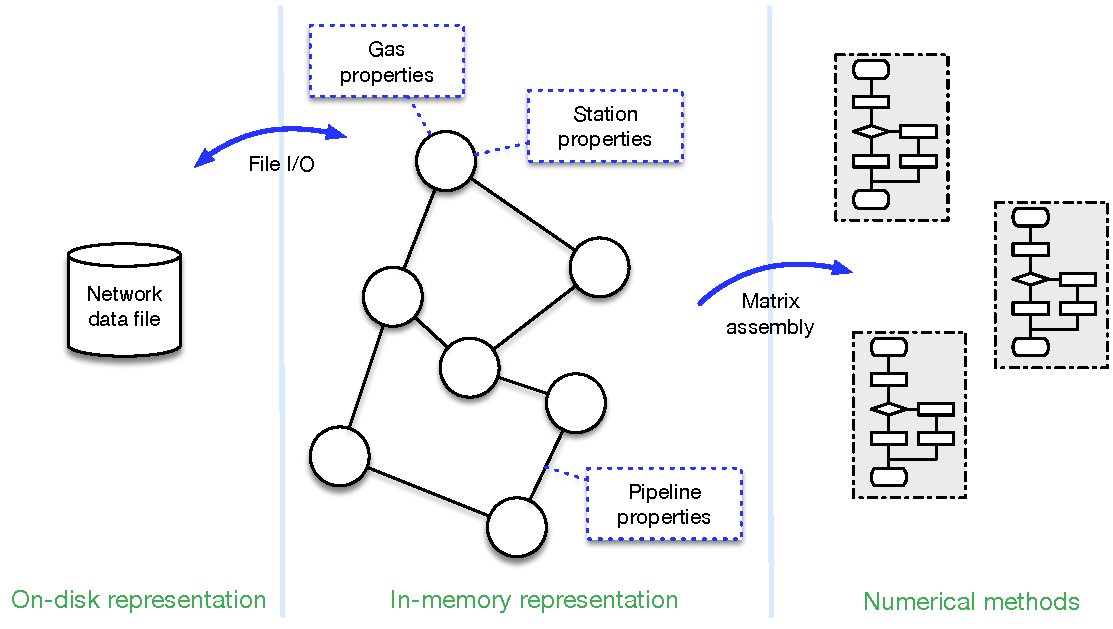
\includegraphics[scale = 0.7]{img_intro/system_arch.pdf}  
    \caption{System architecture scheme.}
    \label{intro:architecture}
\end{figure}

The typical workflow of a Shimmer++ session is as following:
\begin{itemize}
    \item Create an empty NDF based on the Shimmer++ database schema
    \item Populate the NDF with the network data (either manually or from other codes)
    \item Provide a small configuration file with the simulation parameters
    \item Run the tool
    \item Read the results from the NDF and postprocess them with the appropriate software
\end{itemize}
